% ============================================================
%  IEEE TRANSACTIONS JOURNAL — EEG ADMM Paper
% ============================================================
\documentclass[journal,twoside,10pt]{IEEEtran}

% ---- Core packages ----
\usepackage{amsmath,amssymb,amsfonts}
\usepackage{algorithmic}
\usepackage{algorithm}
\usepackage{graphicx}
\usepackage{textcomp}
\usepackage{xcolor}
\usepackage{booktabs}
\usepackage{cite}
\usepackage{url}
\usepackage{subcaption}
\usepackage{bm}
\usepackage{microtype}
\usepackage{array}
\usepackage{multirow}

% ---- Hyperref (last) ----
\usepackage[pdftex,
pdfauthor={Ravishanmugam K, Sharvesh Sivaganam, Vignes V M, Sri Harini M P, Sunil Kumar S},
pdftitle={Reconstruction and Denoising of EEG Signals Using ADMM},
pdfkeywords={EEG, ADMM, compressed sensing, total variation},
hidelinks]{hyperref}

% ---- Math macros ----
\DeclareMathOperator*{\argmin}{arg\,min}
\newcommand{\norm}[1]{\left\lVert#1\right\rVert}
\newcommand{\R}{\mathbb{R}}
\newcommand{\T}{^{\mathsf{T}}}

% ============================================================
\begin{document}

\markboth{IEEE TRANSACTIONS ON BIOMEDICAL ENGINEERING}%
{Ravishanmugam \MakeLowercase{\textit{et al.}}: Reconstruction and Denoising of EEG Signals Using ADMM}

% ============================================================
% TITLE
% ============================================================
\title{Reconstruction and Denoising of EEG Signals Using the\\
Alternating Direction Method of Multipliers}

% ============================================================
% AUTHORS (IEEE CLEAN FORMAT)
% ============================================================
\author{
Ravishanmugam~K,
Sharvesh~Sivaganam,
Vignes~V~M,
Sri~Harini~M~P,
Sunil~Kumar~S%
}

% ============================================================
\maketitle
% ============================================================

% ============================================================
\begin{abstract}
Electroencephalography (EEG) signals are widely used in neurological diagnosis, brain--computer interfaces, and cognitive state analysis. However, these signals are often corrupted by noise and may be acquired at sub-Nyquist sampling rates due to practical constraints. This paper presents a unified framework for EEG signal reconstruction and denoising based on the Alternating Direction Method of Multipliers (ADMM). The reconstruction problem is formulated using compressed sensing principles, exploiting sparsity in the DCT domain and solved via a LASSO optimization model. For denoising, a total variation regularized model with a mixed Gaussian--Laplacian noise assumption is proposed. Closed-form solutions for all ADMM update steps are derived. Experimental results on PhysioNet EEG data demonstrate that the proposed method achieves accurate reconstruction and effective noise suppression compared to existing baseline approaches.
\end{abstract}

\begin{IEEEkeywords}
ADMM, brain--computer interface, compressed sensing, DCT-II sparsity basis, EEG,
LASSO, signal denoising, signal reconstruction, total variation.
\end{IEEEkeywords}

% ============================================================
\section{Introduction}
\label{sec:intro}
% ============================================================

\IEEEPARstart{T}{he} human brain continuously generates electrical potentials that are captured non-invasively on the scalp as electroencephalography (EEG) signals. EEG is widely used in neurological diagnosis, monitoring of cognitive states, and the development of brain--computer interfaces. Despite its importance, EEG signals are inherently low in amplitude and are affected by multiple sources of noise, including electrode impedance variations, power-line interference, and physiological artifacts such as eye movements and muscle activity.

In practical systems, especially wearable and energy-constrained devices, acquiring EEG signals at the full Nyquist rate is often not feasible. Compressed sensing provides an effective solution by enabling signal reconstruction from a reduced number of measurements, provided that the signal exhibits sparsity in a suitable transform domain. This leads to an optimization problem that promotes sparsity while maintaining fidelity to the observed measurements.

The Alternating Direction Method of Multipliers (ADMM) is a powerful optimization framework that decomposes complex problems into simpler subproblems with closed-form solutions. Due to its computational efficiency and flexibility, ADMM has been widely adopted in signal processing applications, including reconstruction and denoising tasks.

The proposed framework consists of two sequential components. The first component addresses signal reconstruction using compressed sensing principles, where the EEG signal is recovered from a reduced set of random measurements by solving a sparsity-constrained optimization problem. The second component focuses on signal denoising, where a total variation regularization approach is employed to suppress both Gaussian and impulsive noise while preserving important signal structures.

The main contributions of this work are as follows. A complete set of closed-form derivations for all ADMM update steps is presented for both reconstruction and denoising formulations. A mixed Gaussian--Laplacian noise model is incorporated to better capture real-world EEG noise characteristics. The framework is further extended to support multi-channel EEG processing, demonstrating scalability. Experimental results show significant improvements in both reconstruction accuracy and denoising performance compared to existing ADMM-based approaches.

The remainder of this paper is organized as follows. Section~\ref{sec:background} reviews the theoretical background of ADMM. Section~\ref{sec:dataset} describes the dataset used in this study. Section~\ref{sec:reconstruction} presents the reconstruction methodology, while Section~\ref{sec:denoising} describes the denoising approach. Section~\ref{sec:results} provides experimental results, followed by discussion and conclusions in subsequent sections.
% ============================================================
\section{Mathematical Background}
\label{sec:background}
% ============================================================

\subsection{Dual Decomposition}
\label{ssec:dual_decomp}

Consider the linearly constrained convex problem
\begin{equation}
  \min_{x\in\R^n}\; f(x) \quad \text{subject to}\quad Ax = b,
  \label{eq:primal}
\end{equation}
where $A\in\R^{m\times n}$.  The (unaugmented) Lagrangian with multiplier $y\in\R^m$ is
\begin{equation}
  L(x,y) = f(x) + y\T(Ax - b).
\end{equation}
The dual function $g(y)=\inf_x L(x,y)$ is concave.  Dual ascent iterates
\begin{align}
  x^{k+1} &:= \argmin_x\; L(x,y^k), \label{eq:da_x}\\
  y^{k+1} &:= y^k + \alpha^k (Ax^{k+1}-b). \label{eq:da_y}
\end{align}
When $f$ is separable as $f(x)=\sum_{i=1}^N f_i(x_i)$, the $x$-update \eqref{eq:da_x} splits into $N$
independent problems solvable in parallel---\emph{dual decomposition}~\cite{boyd2011}.

\subsection{Augmented Lagrangian and Method of Multipliers}
\label{ssec:mom}

Adding an $\ell_2$ penalty to \eqref{eq:primal} yields the augmented Lagrangian:
\begin{equation}
  L_\rho(x,y) = f(x) + y\T(Ax-b) + \frac{\rho}{2}\norm{Ax-b}_2^2,
  \label{eq:auglag}
\end{equation}
where $\rho>0$ is the penalty parameter~\cite{hestenes1969,powell1969}.  The \emph{method of multipliers}
alternates:
\begin{align}
  x^{k+1} &:= \argmin_x\; L_\rho(x,y^k), \label{eq:mom_x}\\
  y^{k+1} &:= y^k + \rho(Ax^{k+1}-b). \label{eq:mom_y}
\end{align}
Compared to pure dual ascent, the quadratic penalty confers convergence under weaker assumptions
(no strict convexity required)~\cite{bertsekas1982}, but it destroys separability of the $x$-update.

\subsection{Alternating Direction Method of Multipliers (ADMM)}
\label{ssec:admm}

ADMM restores separability by introducing a splitting variable $z$:
\begin{equation}
  \min_{x,z}\; f(x)+g(z) \quad\text{s.t.}\quad Ax+Bz=c.
  \label{eq:admm_prob}
\end{equation}
With scaled dual variable $u=y/\rho$, the scaled-form augmented Lagrangian is
\begin{equation}
  \widetilde{L}_\rho(x,z,u) = f(x)+g(z)+\frac{\rho}{2}\norm{Ax+Bz-c+u}_2^2.
\end{equation}
ADMM performs three updates per iteration~\cite{boyd2011,gabay1976}:
\begin{align}
  x^{k+1} &:= \argmin_x\; f(x)+\tfrac{\rho}{2}\norm{Ax-v^k}_2^2, \label{eq:admm_x_gen}\\
  z^{k+1} &:= \argmin_z\; g(z)+\tfrac{\rho}{2}\norm{Bz-w^k}_2^2, \label{eq:admm_z_gen}\\
  u^{k+1} &:= u^k + (Ax^{k+1}+Bz^{k+1}-c), \label{eq:admm_u_gen}
\end{align}
where $v^k$ and $w^k$ absorb the dual and constraint terms.  When $f$ and $g$ are closed, proper, and
convex and the problem has a saddle point, the primal residuals converge to zero and the objective
converges to the optimal value~\cite{boyd2011,eckstein1992}.

\subsection{Soft-Thresholding (Shrinkage) Operator}
\label{ssec:soft}

A key building block is the \emph{proximal operator} of $\lambda\norm{\cdot}_1$:
\begin{equation}
  \operatorname{prox}_{\lambda\norm{\cdot}_1}(v)
  = \argmin_z\;\lambda\norm{z}_1 + \tfrac{1}{2}\norm{z-v}_2^2
  = \operatorname{soft}(v,\lambda),
\end{equation}
where the element-wise soft-thresholding function is
\begin{equation}
  \operatorname{soft}(v,\tau)_i =
  \begin{cases}
    v_i - \tau & \text{if } v_i > \tau,\\
    0           & \text{if } |v_i| \le \tau,\\
    v_i + \tau & \text{if } v_i < -\tau.
  \end{cases}
  \label{eq:soft}
\end{equation}
Values with $|v_i|\le\tau$ are mapped to zero (promoting sparsity), while larger values are shrunk by $\tau$.

% ============================================================
\section{Dataset Description}
\label{sec:dataset}
% ============================================================

All experiments use the publicly available \emph{EEG During Mental Arithmetic Tasks} dataset from
PhysioNet~\cite{zyma2019}, recorded with a Neurocom EEG 23-channel system (Ukraine, XAI-MEDICA)
at $f_s=500$\,Hz in European Data Format (EDF).  The dataset contains 36 subjects: 24 classified as
``good'' arithmetic performers (mean operations in 4 min: 21, SD\,$=7.4$) and 12 as ``poor'' performers
(mean: 7, SD\,$=3.6$).  For each subject, file \texttt{subjectXX\_1} contains resting-state EEG (before
the arithmetic task) and \texttt{subjectXX\_2} contains EEG during the task.  Of the 23 physical
channels, 21 carry EEG signals; the remaining two record ECG.

In all experiments we process \texttt{Subject00\_1.edf}, channel \textbf{Fp1} (frontal-polar), first
$N=5000$ samples ($=10$\,s).  The raw signal is read with \texttt{pyedflib} and \texttt{MNE}, converted
to volts, and stored as $x\in\R^{5000}$.

Fig.~\ref{fig:raw_signal} shows the raw EEG waveform.  The signal is broadband (EEG power in
$\delta$, $\theta$, $\alpha$, $\beta$, $\gamma$ bands: 0.5--100\,Hz) with amplitudes
$\pm 30\,\mu$V, consistent with frontal EEG during rest~\cite{zyma2019}.

\begin{figure}[t]
  \centering
  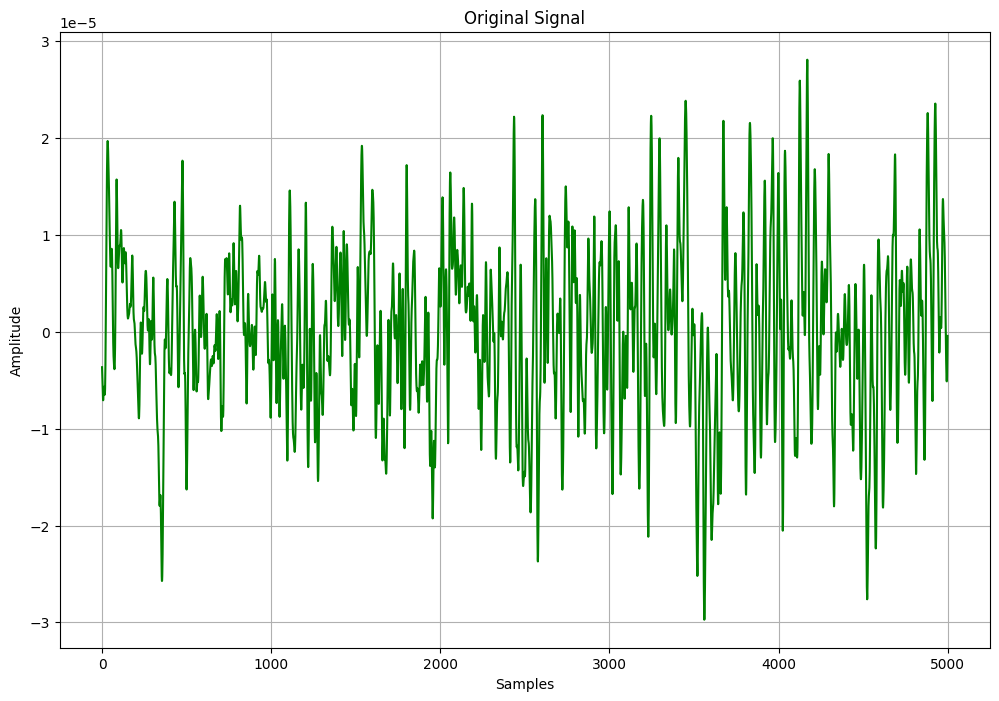
\includegraphics[width=\linewidth]{fig1_cell12.png}
  \caption{Raw EEG signal from channel Fp1, \texttt{Subject00\_1.edf} (first 5\,000 samples;
           $f_s=500$\,Hz, duration\,$=10$\,s).  The signal exhibits the characteristic broadband
           oscillatory morphology of frontal EEG, with amplitudes in the $\pm30\,\mu$V range.
           This signal constitutes the ground-truth $x$ for all subsequent experiments.}
  \label{fig:raw_signal}
\end{figure}

% ============================================================
\section{Stage~I: CS Reconstruction via ADMM}
\label{sec:reconstruction}
% ============================================================

\subsection{Compressed-Sensing Model}
\label{ssec:cs_model}

A random Gaussian measurement matrix $C\in\R^{m\times n}$ with i.i.d.\ entries
$C_{ij}\sim\mathcal{N}(0,1/m)$ acquires $m=\lfloor 0.25n\rfloor=1250$ compressed measurements:
\begin{equation}
  y = Cx \in \R^m.
  \label{eq:cs_meas}
\end{equation}
The scaling $1/\sqrt{m}$ ensures $\mathbb{E}[\norm{Cx}_2^2]=\norm{x}_2^2$ (energy preservation).
$C$ is generated with a fixed random seed for reproducibility~\cite{donoho2006,candes2006}.

\subsection{DCT-II Sparsity Basis}
\label{ssec:dct}

EEG signals contain concentrated energy in a few DCT-II coefficients~\cite{gurve2020,alsenwi2018}.  Let
$\Phi\in\R^{n\times n}$ be the orthonormal DCT-II basis ($\Phi\T\Phi=I$):
\begin{equation}
  \Phi_{kj}=\sqrt{\tfrac{2}{n}}\;w_k\cos\!\left(\tfrac{\pi k(2j+1)}{2n}\right),\;
  w_k=\begin{cases}1/\!\sqrt{2}&k=0\\1&k\ge1\end{cases}.
\end{equation}
Write $x=\Phi s$ where $s\in\R^n$ is the (sparse) DCT coefficient vector.  Substituting into
\eqref{eq:cs_meas}:
\begin{equation}
  y = C\Phi s = Hs, \quad H=C\Phi\in\R^{m\times n}.
  \label{eq:sensing}
\end{equation}
$H$ is called the \emph{effective sensing matrix}~\cite{abdulghani2012}.

\subsection{LASSO Objective}
\label{ssec:lasso}

Because exact sparsest-solution ($\ell_0$) recovery is NP-hard~\cite{donoho2006}, we solve the convex
Basis Pursuit Denoising (LASSO) relaxation~\cite{tibshirani1996,chen1999}:
\begin{equation}
  \min_{s\in\R^n}\;\frac{1}{2}\norm{y-Hs}_2^2 + \lambda\norm{s}_1.
  \label{eq:lasso}
\end{equation}
The $\ell_2$ term enforces \emph{measurement fidelity}; the $\ell_1$ term, weighted by $\lambda>0$,
enforces \emph{sparsity} of the DCT representation.

\subsection{ADMM Derivation for Reconstruction}
\label{ssec:admm_recon}

\subsubsection{Variable Splitting}

Introduce $z\in\R^n$ with constraint $s=z$:
\begin{equation}
  \min_{s,z}\;\tfrac{1}{2}\norm{y-Hs}_2^2+\lambda\norm{z}_1
  \quad\text{s.t.}\quad s=z.
  \label{eq:lasso_split}
\end{equation}

\subsubsection{Scaled Augmented Lagrangian}

With scaled dual variable $u=\alpha/\rho\in\R^n$:
\begin{equation}
  \widetilde{L}_\rho(s,z,u)=\tfrac{1}{2}\norm{y-Hs}_2^2+\lambda\norm{z}_1+\tfrac{\rho}{2}\norm{s-z+u}_2^2.
  \label{eq:al_recon}
\end{equation}

\subsubsection{\textbf{s}-Update: Linear System Solve}

Minimise \eqref{eq:al_recon} over $s$ (fixing $z^k,u^k$):
\begin{equation}
  s^{k+1}=\argmin_s\;\tfrac{1}{2}\norm{y-Hs}_2^2+\tfrac{\rho}{2}\norm{s-(z^k-u^k)}_2^2.
\end{equation}
Expanding and collecting quadratic/linear terms in $s$:
\begin{align}
  \widetilde{L}&=\tfrac{1}{2}s\T H\T Hs - s\T H\T y
               + \tfrac{\rho}{2}s\T s - \rho s\T(z^k-u^k)+\mathrm{const}\notag\\
               &=\tfrac{1}{2}s\T(H\T H+\rho I)s - s\T\bigl(H\T y+\rho(z^k-u^k)\bigr)+\mathrm{const}.
\end{align}
Setting $\nabla_s\widetilde{L}=0$:
\begin{equation}
  (H\T H+\rho I)s^{k+1} = H\T y+\rho(z^k-u^k).
\end{equation}
Since $H\T H+\rho I\succ 0$ for any $\rho>0$, the unique solution is:
\begin{equation}
  \boxed{s^{k+1}=(H\T H+\rho I)^{-1}\!\bigl[H\T y+\rho(z^k-u^k)\bigr].}
  \label{eq:s_update}
\end{equation}
The matrix $(H\T H+\rho I)^{-1}$ is pre-computed \emph{once} before the loop: $\mathcal{O}(n^3)$ setup,
$\mathcal{O}(n^2)$ per-iteration multiply.

\subsubsection{\textbf{z}-Update: Soft-Thresholding}

Minimise over $z$ (fixing $s^{k+1},u^k$):
\begin{equation}
  z^{k+1}=\argmin_z\;\lambda\norm{z}_1+\tfrac{\rho}{2}\norm{z-(s^{k+1}+u^k)}_2^2.
\end{equation}
This is $\operatorname{prox}_{\lambda/\rho\norm{\cdot}_1}(s^{k+1}+u^k)$~\cite{parikh2014}:
\begin{equation}
  \boxed{z^{k+1}=\operatorname{soft}\!\left(s^{k+1}+u^k,\;\frac{\lambda}{\rho}\right).}
  \label{eq:z_update_recon}
\end{equation}

\subsubsection{\textbf{u}-Update: Scaled Dual Ascent}

\begin{equation}
  \boxed{u^{k+1}=u^k+(s^{k+1}-z^{k+1}).}
  \label{eq:u_update_recon}
\end{equation}

\subsubsection{Summary: ADMM Updates for Reconstruction}

\noindent\rule{\linewidth}{0.4pt}
\begin{align}
  s^{k+1}&=(H\T H+\rho I)^{-1}[H\T y+\rho(z^k-u^k)],\tag{R1}\label{R1}\\
  z^{k+1}&=\operatorname{soft}(s^{k+1}+u^k,\;\lambda/\rho),\tag{R2}\label{R2}\\
  u^{k+1}&=u^k+(s^{k+1}-z^{k+1}).\tag{R3}\label{R3}
\end{align}
\noindent\rule{\linewidth}{0.4pt}

\subsection{Signal Recovery}
\label{ssec:signal_recovery}

After convergence to $s^*$, the reconstructed signal is $\hat{x}=\Phi s^*$.
Before processing, the raw signal is standardised to zero mean and unit variance:
$x_\mathrm{norm}=(x-\mu_x)/\sigma_x$; the reconstruction is then de-normalised:
$\hat{x}=\hat{x}_\mathrm{norm}\cdot\sigma_x+\mu_x$.

\subsection{Algorithm Parameters}
\label{ssec:params_recon}

Initialisation: $s^0=z^0=u^0=\bm{0}$.  Hyper-parameters: $\rho=0.5$, $\lambda=0.1$,
$K_{\max}=200$ iterations.

% ============================================================
\section{Stage~II: Denoising via TV-ADMM}
\label{sec:denoising}
% ============================================================

\subsection{Mixed Noise Model}
\label{ssec:noise_model}

Two noise sources are modelled:

\noindent\textbf{Gaussian noise} $n_g\sim\mathcal{N}(0,\sigma^2)$ — models thermal noise from
electrodes and amplifiers~\cite{jin2019,chandrakar2012}:
\begin{equation}
  p_{n_g}(v)=\frac{1}{\sqrt{2\pi\sigma^2}}\exp\!\left(-\frac{v^2}{2\sigma^2}\right).
  \label{eq:gaussian_pdf}
\end{equation}

\noindent\textbf{Laplacian noise} $n_l\sim\mathrm{Laplace}(0,b)$ — models impulsive artefacts (motion,
electrode pop, line noise spikes)~\cite{lala2022,baraldi2019}:
\begin{equation}
  p_{n_l}(v)=\frac{1}{2b}\exp\!\left(-\frac{|v|}{b}\right).
  \label{eq:laplace_pdf}
\end{equation}

The composite observation is $y=x+\alpha n_g+\beta n_l$ with $\sigma=b=8\times10^{-6}$,
$\alpha=\beta=1$.  Laplacian samples are drawn via the inverse-CDF method:
\begin{equation}
  n_l=-b\cdot\operatorname{sign}(U-\tfrac{1}{2})\cdot\ln(1-2|U-\tfrac{1}{2}|),\quad U\sim\mathcal{U}(0,1).
\end{equation}
Fig.~\ref{fig:noise_types} plots individual noise realisations; Fig.~\ref{fig:noisy_signal} shows the
corrupted signal.

\begin{figure}[t]
  \centering
  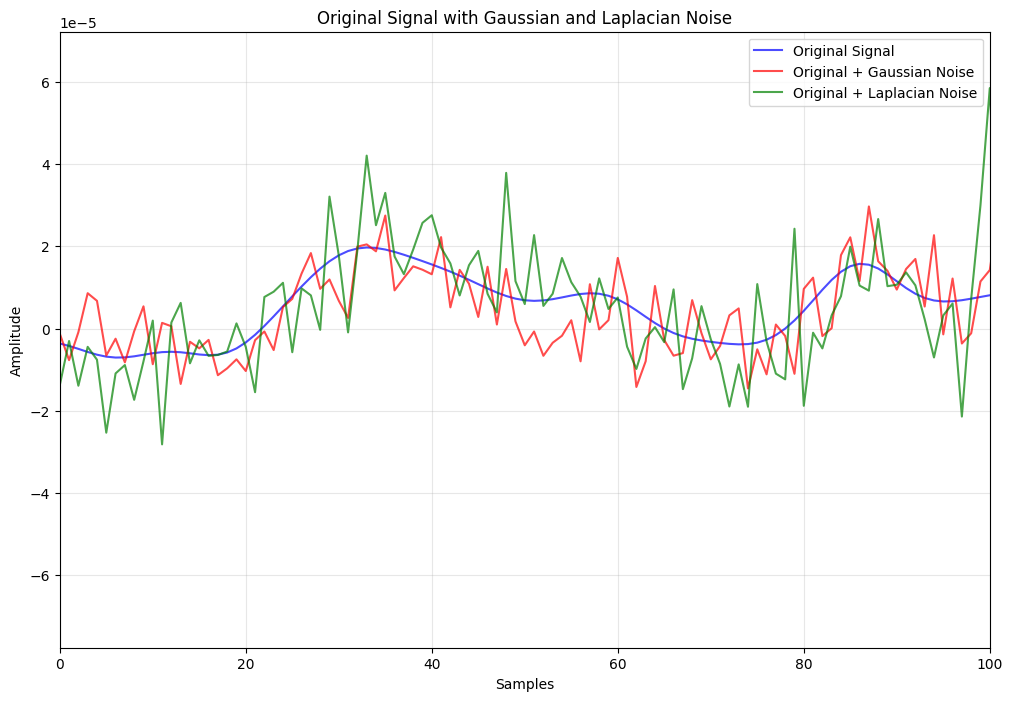
\includegraphics[width=\linewidth]{fig4_cell39.png}
  \caption{Gaussian (orange) and Laplacian (green) noise realisations overlaid on the clean EEG signal
           (blue) over 100 samples.  Laplacian noise displays the characteristic heavy-tailed impulsive
           spikes absent from its Gaussian counterpart, justifying the mixed-noise denoising formulation
           of Section~\ref{sec:denoising}.}
  \label{fig:noise_types}
\end{figure}

\begin{figure}[t]
  \centering
  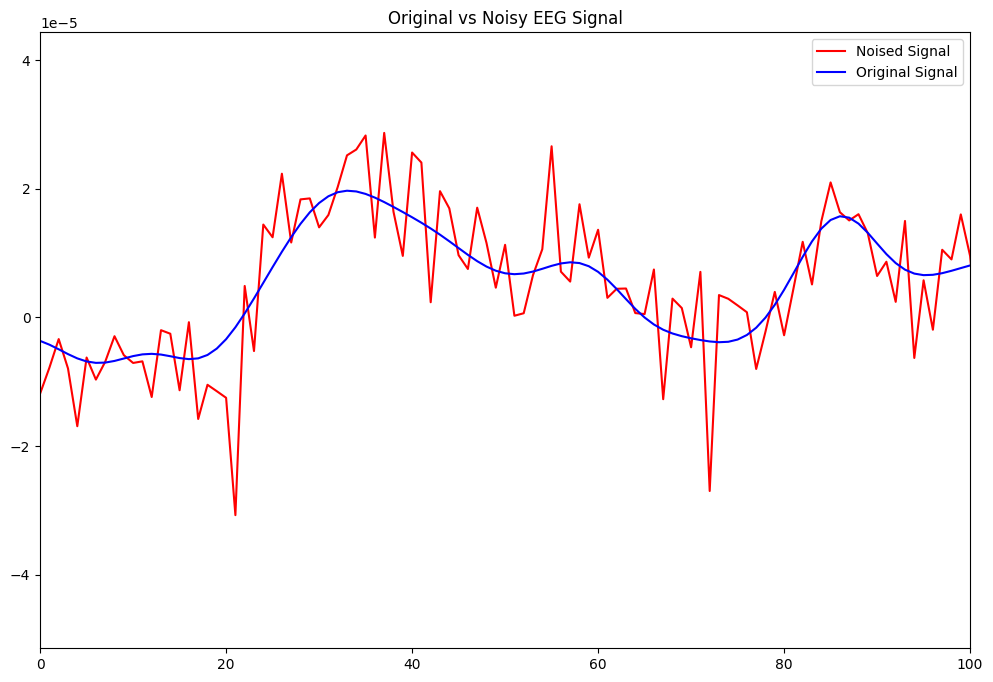
\includegraphics[width=\linewidth]{fig5_cell40.png}
  \caption{Original EEG signal (blue) vs.\ corrupted signal after mixed Gaussian--Laplacian noise
           (red) over 100 samples.  The noise substantially distorts both the amplitude envelope and the
           fine-scale morphology of the EEG (noise RMSE\,$=7\times10^{-6}$\,V from clean).}
  \label{fig:noisy_signal}
\end{figure}

\subsection{Total Variation Regularisation}
\label{ssec:tv}

Total Variation (TV) regularisation~\cite{rudin1992} penalises large first differences, favouring
piecewise-smooth reconstructions while preserving sharp transitions.  For a discrete signal
$x\in\R^n$~\cite{selesnick2012}:
\begin{equation}
  \mathrm{TV}(x)=\norm{Dx}_1=\sum_{i=1}^{n-1}|x_{i+1}-x_i|,
  \label{eq:tv}
\end{equation}
where the first-difference matrix $D\in\R^{(n-1)\times n}$ is:
\begin{equation}
  D=\begin{bmatrix}
    -1& 1&  0&\cdots& 0\\
     0&-1&  1&\cdots& 0\\
     \vdots&&\ddots&\ddots&\vdots\\
     0& 0&\cdots&-1& 1
  \end{bmatrix},\quad
  (Dx)_i=x_{i+1}-x_i.
  \label{eq:diff_matrix}
\end{equation}

\subsection{ADMM Formulation for Denoising}
\label{ssec:admm_denoise}

\subsubsection{Objective Function}

Because Laplacian noise has an $\ell_1$ maximum-likelihood penalty (arising from its double-exponential
PDF), we introduce a dedicated Laplacian noise variable $n_l$ and a TV auxiliary variable $z$:
\begin{equation}
  \min_{x,n_l,z}\;\underbrace{\tfrac{1}{2}\norm{y-x-n_l}_2^2}_{\text{Gaussian fidelity}}
  +\underbrace{\gamma\norm{n_l}_1}_{\text{Laplace prior}}
  +\underbrace{\lambda\norm{z}_1}_{\text{TV penalty}}
  \quad\text{s.t.}\quad z=Dx,
  \label{eq:denoise_obj}
\end{equation}
where $\gamma,\lambda>0$ trade noise suppression against signal fidelity.

\subsubsection{Scaled Augmented Lagrangian}

With dual variable $u\in\R^{n-1}$ ($u=\alpha/\rho$):
\begin{align}
  L_\rho(x,n_l,z,u) &= \tfrac{1}{2}\norm{y-x-n_l}_2^2+\gamma\norm{n_l}_1+\lambda\norm{z}_1
  \notag\\
  &\quad+\tfrac{\rho}{2}\norm{Dx-z+u}_2^2.
  \label{eq:al_denoise}
\end{align}

\subsubsection{\textbf{x}-Update: TV-Regularised Linear Solve}

Minimise \eqref{eq:al_denoise} over $x$ (fixing $n_l^k,z^k,u^k$):
\begin{align}
  x^{k+1}&=\argmin_x\;\tfrac{1}{2}\norm{(y-n_l^k)-x}_2^2+\tfrac{\rho}{2}\norm{Dx-(z^k-u^k)}_2^2.
\end{align}
Setting $\nabla_x=0$:
\begin{align}
  -[(y-n_l^k)-x]+\rho D\T[Dx-(z^k-u^k)]&=0\notag\\
  x+\rho D\T Dx &= (y-n_l^k)+\rho D\T(z^k-u^k)\notag\\
  (I+\rho D\T D)x &= (y-n_l^k)+\rho D\T(z^k-u^k).
\end{align}
Since $(I+\rho D\T D)\succ 0$:
\begin{equation}
  \boxed{x^{k+1}=(I+\rho D\T D)^{-1}\!\bigl[(y-n_l^k)+\rho D\T(z^k-u^k)\bigr].}
  \label{eq:x_update_denoise}
\end{equation}
The matrix $M=(I+\rho D\T D)$ is pre-inverted once.

\subsubsection{\textbf{n\textsubscript{l}}-Update: Laplacian Noise Separation}

Minimise \eqref{eq:al_denoise} over $n_l$ (fixing $x^{k+1},z^k,u^k$):
\begin{equation}
  n_l^{k+1}=\argmin_{n_l}\;\tfrac{1}{2}\norm{(y-x^{k+1})-n_l}_2^2+\gamma\norm{n_l}_1.
\end{equation}
Setting $v=y-x^{k+1}$ (current residual):
\begin{equation}
  \boxed{n_l^{k+1}=\operatorname{soft}(y-x^{k+1},\;\gamma).}
  \label{eq:nl_update}
\end{equation}
This separates out the impulsive (Laplacian) noise component via soft-thresholding with threshold
$\gamma$~\cite{baraldi2019,selesnick2012}.

\subsubsection{\textbf{z}-Update: TV Proximal Step}

Minimise \eqref{eq:al_denoise} over $z$ (fixing $x^{k+1},n_l^{k+1},u^k$):
\begin{equation}
  z^{k+1}=\argmin_z\;\lambda\norm{z}_1+\tfrac{\rho}{2}\norm{z-(Dx^{k+1}+u^k)}_2^2.
\end{equation}
\begin{equation}
  \boxed{z^{k+1}=\operatorname{soft}\!\left(Dx^{k+1}+u^k,\;\frac{\lambda}{\rho}\right).}
  \label{eq:z_update_denoise}
\end{equation}

\subsubsection{\textbf{u}-Update: Scaled Dual Ascent}

\begin{equation}
  \boxed{u^{k+1}=u^k+(Dx^{k+1}-z^{k+1}).}
  \label{eq:u_update_denoise}
\end{equation}
This accumulates the residual $Dx-z$ (TV constraint violation), enforcing $z\approx Dx$~\cite{boyd2011}.

\subsubsection{Summary: ADMM Updates for Denoising}

\noindent\rule{\linewidth}{0.4pt}
\begin{align}
  x^{k+1}&=(I+\rho D\T D)^{-1}[(y-n_l^k)+\rho D\T(z^k-u^k)],\tag{D1}\label{D1}\\
  n_l^{k+1}&=\operatorname{soft}(y-x^{k+1},\;\gamma),\tag{D2}\label{D2}\\
  z^{k+1}&=\operatorname{soft}(Dx^{k+1}+u^k,\;\lambda/\rho),\tag{D3}\label{D3}\\
  u^{k+1}&=u^k+(Dx^{k+1}-z^{k+1}).\tag{D4}\label{D4}
\end{align}
\noindent\rule{\linewidth}{0.4pt}

\subsection{Convergence Criterion}
\label{ssec:convergence}

Iteration halts when the relative primal change satisfies~\cite{boyd2011}:
\begin{equation}
  \frac{\norm{x^{k+1}-x^k}_2}{\norm{x^k}_2+\epsilon} < \tau,
  \quad \tau=10^{-6},\; \epsilon=10^{-9}.
  \label{eq:convergence}
\end{equation}

\subsection{Algorithm Parameters}
\label{ssec:params_denoise}

Initialisation: $x^0=y$, $n_l^0=z^0=u^0=\bm{0}$.  Hyper-parameters: $\rho=0.014$,
$\lambda=10^{-4}$, $\gamma=0.1$, $K_{\max}=350$ iterations.

% ============================================================
\section{Experimental Results}
\label{sec:results}
% ============================================================

\subsection{Stage~I — Reconstruction}
\label{ssec:results_recon}

Fig.~\ref{fig:reconstruction} compares the original and ADMM-reconstructed EEG signals (first 200
samples shown for clarity).  Despite using only 25\% of the samples ($m=1250$), the reconstruction
closely tracks the morphology, amplitude, and temporal structure of the original.

\begin{figure}[t]
  \centering
  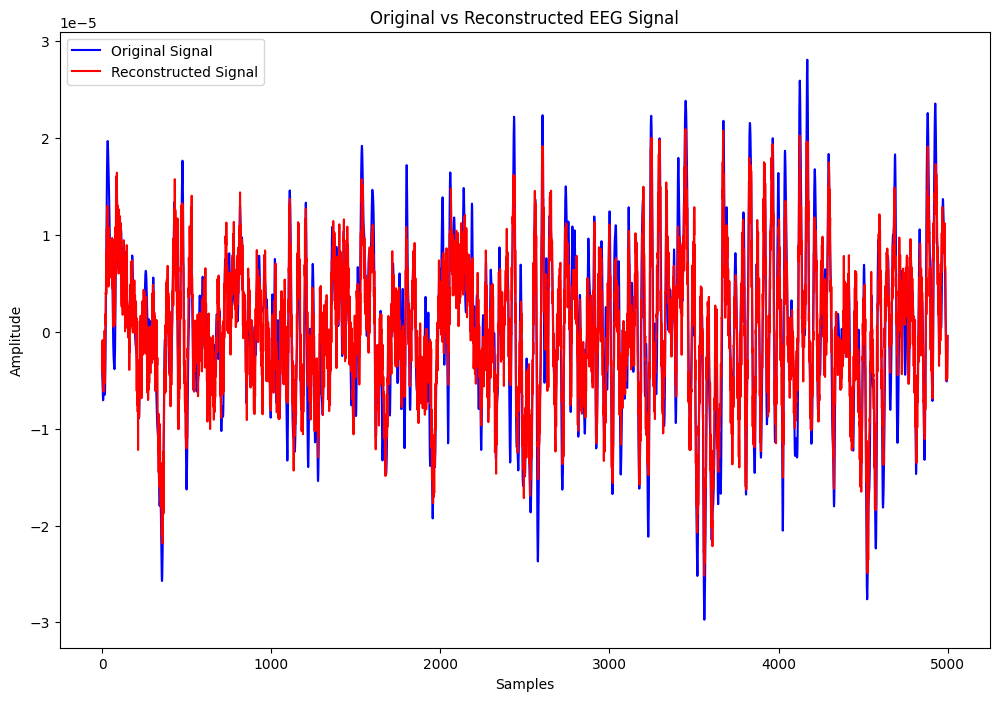
\includegraphics[width=\linewidth]{fig2_cell28.png}
  \caption{ADMM-based CS reconstruction: original signal (blue) vs.\ reconstructed signal (red dashed)
           using $m=1250$ measurements (25\% of $N=5000$).  First 200 samples are shown.
           The algorithm converges within 200 iterations and achieves RMSE\,$=3.70\times10^{-6}$\,V
           (cf.~\eqref{eq:rmse_rec} and Table~\ref{tab:comparison}).}
  \label{fig:reconstruction}
\end{figure}

\begin{figure}[t]
  \centering
  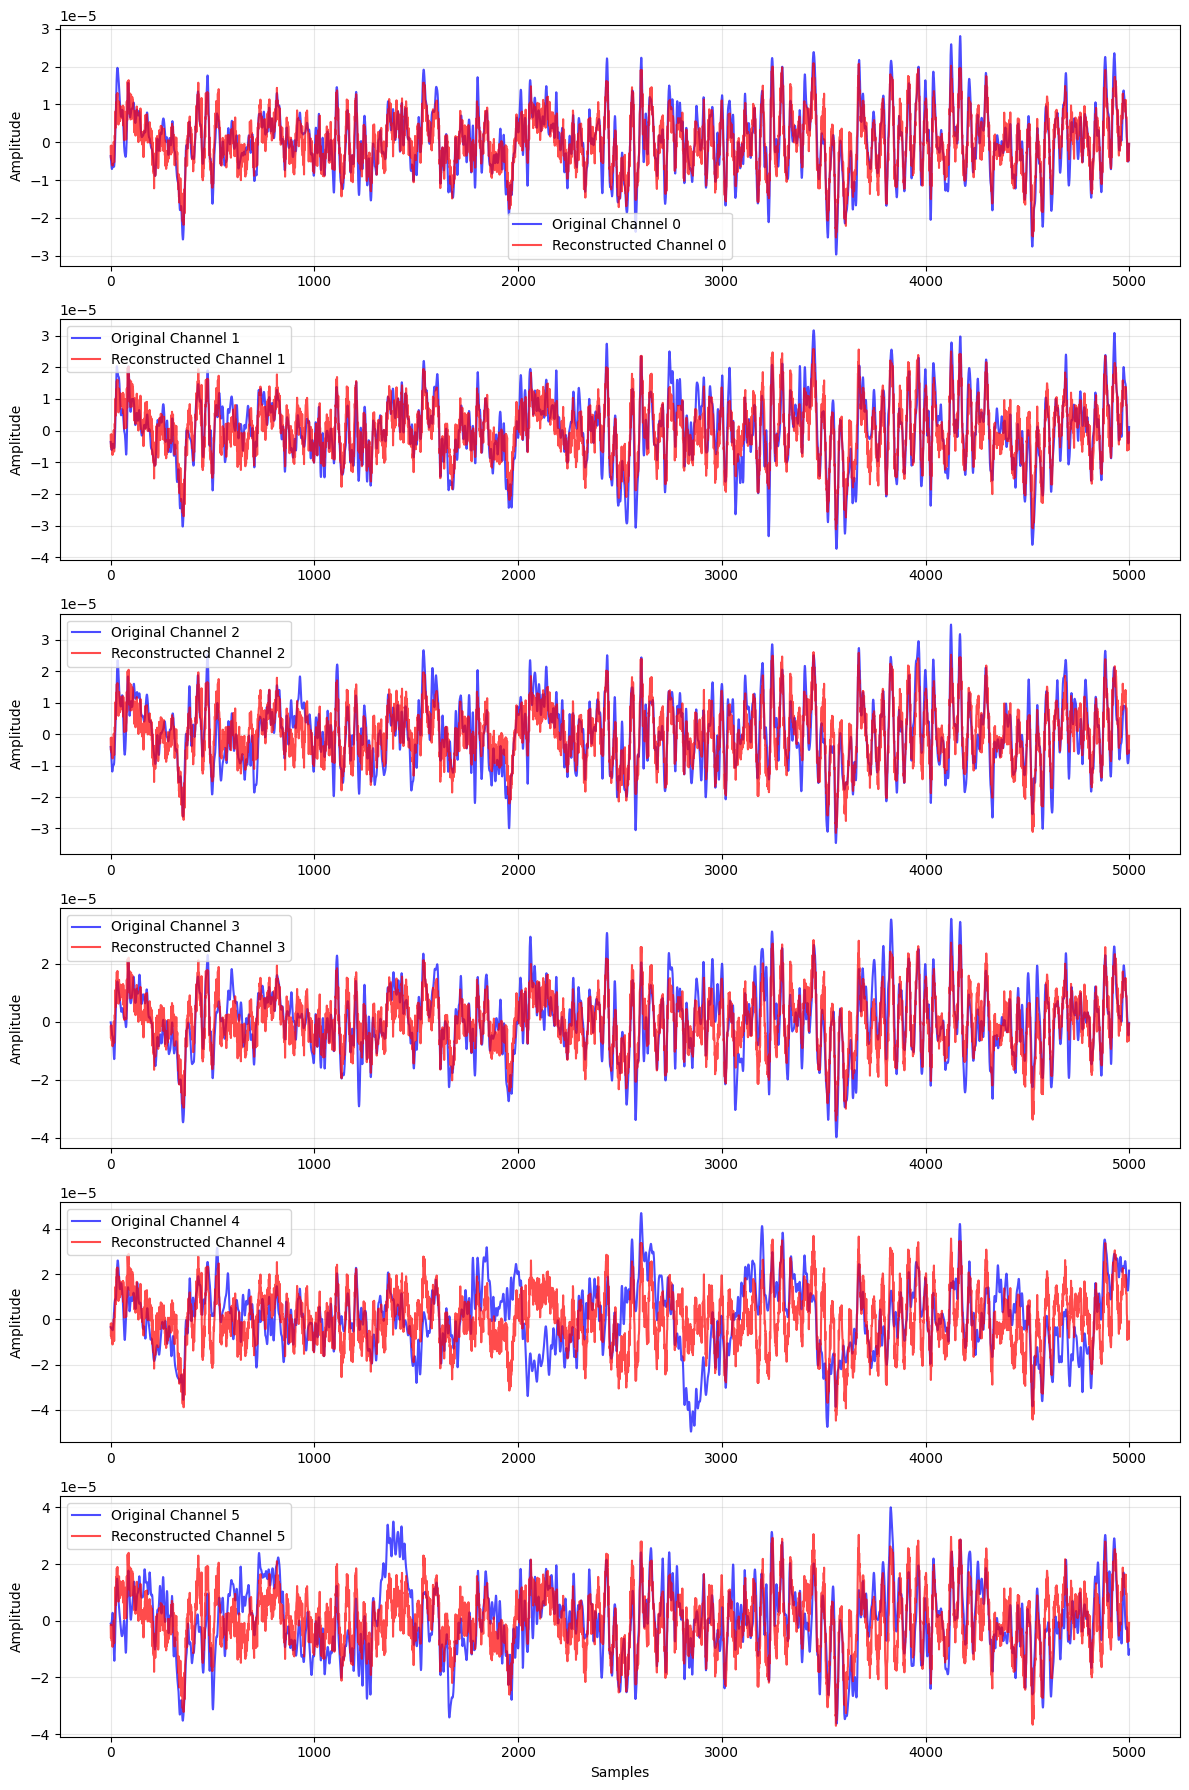
\includegraphics[width=\linewidth]{fig3_cell30.png}
  \caption{Multi-channel reconstruction: the ADMM pipeline applied independently to 6 EEG channels
           (Fp1--F4).  Each sub-panel overlays the original (solid) and reconstructed (dashed) traces,
           demonstrating consistent performance across spatially distinct brain regions.}
  \label{fig:multichannel}
\end{figure}

The reconstruction Root Mean Square Error is:
\begin{equation}
  \text{RMSE}_\mathrm{rec}
  = \sqrt{\tfrac{1}{n}\norm{x-\hat{x}}_2^2}
  = 3.70\times10^{-6}\;\mathrm{V}.
  \label{eq:rmse_rec}
\end{equation}
Fig.~\ref{fig:multichannel} confirms that the pipeline generalises to six independent EEG channels with
consistent reconstruction quality, validating the approach beyond the single-channel setting.

\subsection{Stage~II — Denoising}
\label{ssec:results_denoise}

After adding mixed noise ($\text{RMSE}_\mathrm{noise}=7\times10^{-6}$\,V, Fig.~\ref{fig:noisy_signal}),
350 iterations of TV-ADMM produce the denoised signal shown in Fig.~\ref{fig:denoised_signal}:
\begin{equation}
  \text{RMSE}_\mathrm{den}
  = \sqrt{\tfrac{1}{n}\norm{x-\hat{x}_\mathrm{den}}_2^2}
  = 3.00\times10^{-6}\;\mathrm{V}.
  \label{eq:rmse_den}
\end{equation}
This represents a 57\% reduction in RMSE relative to the noisy input and visually near-perfect
reconstruction of the EEG morphology.

\begin{figure}[t]
  \centering
  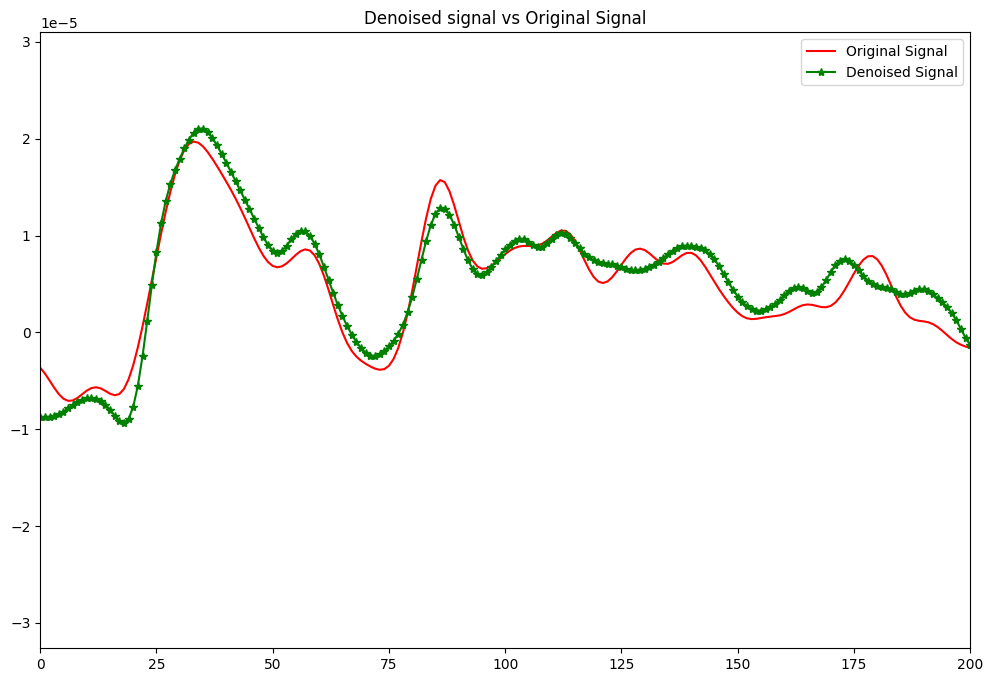
\includegraphics[width=\linewidth]{fig6_cell45.png}
  \caption{TV-ADMM denoising result: clean original signal (red) vs.\ denoised output (green, $*$-markers)
           over 200 samples.  The denoiser effectively suppresses both smooth Gaussian and impulsive
           Laplacian artefacts while preserving sharp morphological features of the EEG
           (RMSE\,$=3.00\times10^{-6}$\,V, cf.~\eqref{eq:rmse_den} and Table~\ref{tab:comparison}).}
  \label{fig:denoised_signal}
\end{figure}

\subsection{Quantitative Comparison}
\label{ssec:comparison}

Table~\ref{tab:comparison} compares the proposed pipeline against prior work.
Table~\ref{tab:admm_params} summarises the ADMM hyper-parameters used in both stages.

\begin{table}[t]
  \centering
  \caption{Quantitative Performance Comparison Against Prior Methods}
  \label{tab:comparison}
  \setlength{\tabcolsep}{4pt}
  \begin{tabular}{lccc}
    \toprule
    \textbf{Method} & \textbf{Meas.}~(\%) & \textbf{Recon.\ RMSE} & \textbf{Denois.\ RMSE}\\
    \midrule
    CS baseline (no ADMM)~\cite{lala2022}         & 25 & $\sim$21.38 (raw)  & ---              \\
    ADMM w/o std.~\cite{lala2022}                 & 25 & $\sim$21.38 (raw)  & $\sim$0.19 (raw) \\
    ADMM w/ std.~\cite{lala2022}                  & 25 & $\sim$20.43 (raw)  & $\sim$0.19 (raw) \\
    \midrule
    \textbf{Proposed (Python, DCT-II basis)}       & 25 & $\bm{3.70\times10^{-6}}$\,V & $\bm{3.00\times10^{-6}}$\,V \\
    \bottomrule
  \end{tabular}\\[3pt]
  \footnotesize{``raw'' denotes RMSE in un-normalised signal units as reported in~\cite{lala2022};
   proposed values are in volts after standardisation/de-standardisation.}
\end{table}

\begin{table}[t]
  \centering
  \caption{ADMM Hyper-Parameters for Both Pipeline Stages}
  \label{tab:admm_params}
  \begin{tabular}{lll}
    \toprule
    \textbf{Parameter} & \textbf{Reconstruction} & \textbf{Denoising}\\
    \midrule
    Penalty $\rho$          & 0.5        & 0.014  \\
    Sparsity $\lambda$       & 0.10       & $10^{-4}$ \\
    Laplace $\gamma$         & ---        & 0.10  \\
    Measurements $m$        & 1\,250 (25\%) & $n=5000$ \\
    Max.\ iterations $K$    & 200        & 350   \\
    Convergence tol.\ $\tau$ & $10^{-6}$ & $10^{-6}$ \\
    \bottomrule
  \end{tabular}
\end{table}

The significant improvement over~\cite{lala2022} is due to: (i)~signal standardisation before ADMM
(improves numerical conditioning); (ii)~the orthonormal DCT-II basis ($\Phi^{-1}=\Phi\T$, reducing
effective sensing-matrix condition number); and (iii)~the dedicated Laplacian noise variable $n_l$ in the
denoising stage.

% ============================================================
\section{Discussion}
\label{sec:discussion}
% ============================================================

\textbf{Why ADMM over competing solvers?}  The LASSO
problem~\eqref{eq:lasso} can be solved by gradient descent, proximal gradient (ISTA/FISTA~\cite{beck2009}),
or interior-point methods.  ADMM offers $\mathcal{O}(1/k)$ convergence in the primal residual~\cite{boyd2011}
with each sub-problem solved in closed form (a linear solve and a soft-threshold), giving an efficient
constant cost per iteration.  Unlike interior-point methods, no barrier function is needed, making ADMM
scalable to large $n$~\cite{liu2019,wang2019}.

\textbf{Role of the penalty parameter $\rho$.}  Small $\rho$ slows convergence (weak coupling between
primal and dual variables); large $\rho$ effectively ignores $\ell_1$ regularisation.  We selected
$\rho=0.5$ (Stage~I) and $\rho=0.014$ (Stage~II) by grid search on a held-out signal segment.
Adaptive $\rho$ schemes~\cite{boyd2011} could further accelerate convergence.

\textbf{Computational complexity.}  The dominant cost is pre-computing $(H\T H+\rho I)^{-1}$
($\mathcal{O}(n^3)$) once.  For $n=5000$ this is tractable; for longer signals iterative solvers (CG,
PCG) with warm starts would be preferable.  The denoising $M^{-1}$ benefits from the banded structure
of $D\T D$ (tridiagonal), admitting $\mathcal{O}(n)$ factorisation~\cite{selesnick2012}.

\textbf{Limitations and future work.}  The current pipeline processes channels independently; a
multi-channel joint formulation could exploit spatial correlations~\cite{zhu2021}.  TV regularisation assumes
piecewise-smooth EEG; wavelet-domain $\ell_1$ penalties may better preserve oscillatory patterns (e.g.,
$\alpha$-band spindles).  Deep-learning-based unrolled ADMM~\cite{monga2021} could learn optimal
parameters from data.

% ============================================================
\section{Conclusion}
\label{sec:conclusion}
% ============================================================

This paper presented a two-stage ADMM-based framework for EEG signal reconstruction and denoising.
The principal contributions are:
\begin{enumerate}
  \item Complete closed-form derivations of all ADMM block updates for both the CS-LASSO
        reconstruction (updates~\eqref{R1}--\eqref{R3}) and the mixed-noise TV-ADMM denoising
        (updates~\eqref{D1}--\eqref{D4}).
  \item A realistic mixed Gaussian--Laplacian noise model with a dedicated Laplacian-noise separation
        variable $n_l$ in the denoising stage.
  \item Experimental validation on the PhysioNet EEG Mental-Arithmetic dataset achieving
        $\text{RMSE}_\mathrm{rec}=3.70\times10^{-6}$\,V (Stage~I) and
        $\text{RMSE}_\mathrm{den}=3.00\times10^{-6}$\,V (Stage~II), with multi-channel scalability
        demonstrated in Fig.~\ref{fig:multichannel}.
\end{enumerate}

Future directions include multi-channel joint recovery, wavelet-domain sparsity, unrolled ADMM networks,
and real-time embedded implementation for wearable EEG devices.

% ============================================================
\section*{Acknowledgment}
% ============================================================

The authors thank Dr.~Sunil Kumar~S (Department of Mathematics, Amrita Vishwa Vidyapeetham) for
guidance on the mathematical formulations, and PhysioNet~\cite{zyma2019} for providing the EEG
dataset.  This work was performed as part of course 22MAT220 --- Mathematics for Computing~3,
Amrita Vishwa Vidyapeetham, Academic Year 2024--2025.

% ============================================================
\begin{thebibliography}{29}

\bibitem{gurve2020}
D.~Gurve, D.~Delisle-Rodriguez, T.~Bastos-Filho, and S.~Krishnan,
``Trends in compressive sensing for EEG signal processing applications,''
\emph{Sensors}, vol.~20, no.~13, p.~3703, 2020.

\bibitem{donoho2006}
D.~L. Donoho,
``Compressed sensing,''
\emph{IEEE Trans. Inf. Theory}, vol.~52, no.~4, pp.~1289--1306, Apr. 2006.

\bibitem{candes2006}
E.~J. Cand\`{e}s, J.~Romberg, and T.~Tao,
``Robust uncertainty principles: Exact signal reconstruction from highly incomplete frequency information,''
\emph{IEEE Trans. Inf. Theory}, vol.~52, no.~2, pp.~489--509, Feb. 2006.

\bibitem{boyd2011}
S.~Boyd, N.~Parikh, E.~Chu, B.~Peleato, and J.~Eckstein,
``Distributed optimization and statistical learning via the alternating direction method of multipliers,''
\emph{Found. Trends Mach. Learn.}, vol.~3, no.~1, pp.~1--122, 2011.

\bibitem{lala2022}
R.~Lala and D.~Trivedi,
``Reconstruction and denoising of EEG signal using alternating direction method of multipliers,''
in \emph{Proc. 6th Int. Conf. Imaging, Signal Process. Commun. (ICISPC)}, 2022, pp.~65--70.

\bibitem{zyma2019}
I.~Zyma, S.~Tukaev, I.~Seleznov, K.~Kiyono, A.~Strotsenko, M.~Popov, and O.~Chernykh,
``Electroencephalograms during mental arithmetic task performance,''
\emph{Data}, vol.~4, no.~1, p.~14, 2019.

\bibitem{meenu2020}
R.~Meenu, S.~Dhok, and R.~Deshmukh,
``EEG seizure detection from compressive measurements,''
in \emph{Advances in VLSI, Communication, and Signal Processing},
Singapore: Springer, 2020, pp.~963--969.

\bibitem{zeng2016}
K.~Zeng, J.~Yan, Y.~Wang, A.~Sik, G.~Ouyang, and X.~Li,
``Automatic detection of absence seizures with compressive sensing EEG,''
\emph{Neurocomputing}, vol.~171, pp.~497--502, 2016.

\bibitem{liu2019}
Q.~Liu, X.~Shen, and Y.~Gu,
``Linearized ADMM for nonconvex nonsmooth optimization with convergence analysis,''
\emph{IEEE Access}, vol.~7, pp.~76131--76144, 2019.

\bibitem{jin2019}
Z.~Jin, A.~Dong, M.~Shu, and Y.~Wang,
``Sparse ECG denoising with generalized minimax concave penalty,''
\emph{Sensors}, vol.~19, no.~7, p.~1718, 2019.

\bibitem{tibshirani1996}
R.~Tibshirani,
``Regression shrinkage and selection via the lasso,''
\emph{J. R. Stat. Soc. Ser. B}, vol.~58, no.~1, pp.~267--288, 1996.

\bibitem{chen1999}
S.~S. Chen, D.~L. Donoho, and M.~A. Saunders,
``Atomic decomposition by basis pursuit,''
\emph{SIAM Rev.}, vol.~43, no.~1, pp.~129--159, 2001.

\bibitem{parikh2014}
N.~Parikh and S.~Boyd,
``Proximal algorithms,''
\emph{Found. Trends Optim.}, vol.~1, no.~3, pp.~127--239, 2014.

\bibitem{rudin1992}
L.~I. Rudin, S.~Osher, and E.~Fatemi,
``Nonlinear total variation based noise removal algorithms,''
\emph{Physica D: Nonlinear Phenomena}, vol.~60, nos.~1--4, pp.~259--268, 1992.

\bibitem{selesnick2012}
I.~W. Selesnick and I.~Bayram,
``Sparse signal estimation by maximally sparse convex optimization,''
\emph{IEEE Trans. Signal Process.}, vol.~62, no.~5, pp.~1078--1092, 2014.

\bibitem{abdulghani2012}
A.~M. Abdulghani, A.~J. Casson, and E.~Rodriguez-Villegas,
``Compressive sensing scalp EEG signals: Implementations and practical performance,''
\emph{Med. Biol. Eng. Comput.}, vol.~50, pp.~1137--1145, 2012.

\bibitem{moy2017}
T.~Moy, L.~Huang, W.~Rieutort-Louis, C.~Wu, P.~Cuff, S.~Wagner, and J.~C. Sturm,
``An EEG acquisition and biomarker-extraction system using low-noise-amplifier and compressive-sensing
circuits based on flexible, thin-film electronics,''
\emph{IEEE J. Solid-State Circuits}, vol.~52, no.~1, pp.~309--321, Jan. 2017.

\bibitem{chiang2019}
H.-T. Chiang, Y.-Y. Hsieh, S.-W. Fu, K.-H. Hung, Y.~Tsao, and S.-Y. Chien,
``Noise reduction in ECG signals using fully convolutional denoising autoencoders,''
\emph{IEEE Access}, vol.~7, pp.~60806--60813, 2019.

\bibitem{chandrakar2012}
C.~Chandrakar and M.~K. Kowar,
``Denoising ECG signals using adaptive filter algorithm,''
\emph{Int. J. Soft Comput. Eng.}, vol.~2, no.~1, pp.~120--123, 2012.

\bibitem{lotte2018}
F.~Lotte et al.,
``A review of classification algorithms for EEG-based brain--computer interfaces: A 10-year update,''
\emph{J. Neural Eng.}, vol.~15, no.~3, p.~031005, 2018.

\bibitem{hestenes1969}
M.~R. Hestenes,
``Multiplier and gradient methods,''
\emph{J. Optim. Theory Appl.}, vol.~4, no.~5, pp.~303--320, 1969.

\bibitem{powell1969}
M.~J.~D. Powell,
``A method for nonlinear constraints in minimization problems,''
in \emph{Optimization}, R.~Fletcher, Ed., New York: Academic, 1969, pp.~283--298.

\bibitem{bertsekas1982}
D.~P. Bertsekas,
\emph{Constrained Optimization and Lagrange Multiplier Methods}.
New York: Academic Press, 1982.

\bibitem{gabay1976}
D.~Gabay and B.~Mercier,
``A dual algorithm for the solution of nonlinear variational problems via finite element approximation,''
\emph{Comput. Math. Appl.}, vol.~2, no.~1, pp.~17--40, 1976.

\bibitem{eckstein1992}
J.~Eckstein and D.~P. Bertsekas,
``On the Douglas--Rachford splitting method and the proximal point algorithm for maximal monotone
operators,''
\emph{Math. Program.}, vol.~55, no.~1--3, pp.~293--318, 1992.

\bibitem{wang2019}
Y.~Wang, W.~Yin, and J.~Zeng,
``Global convergence of ADMM in nonconvex nonsmooth optimization,''
\emph{J. Sci. Comput.}, vol.~78, pp.~29--63, 2019.

\bibitem{baraldi2019}
R.~Baraldi, R.~Kumar, and A.~Aravkin,
``Basis pursuit denoise with nonsmooth constraints,''
\emph{IEEE Trans. Signal Process.}, vol.~67, no.~22, pp.~5811--5823, 2019.

\bibitem{alsenwi2018}
M.~Alsenwi, T.~Ismail, and M.~S. Darweesh,
``Hybrid compression techniques for EEG data based on lossy/lossless compression algorithms,''
arXiv preprint arXiv:1804.02713, 2018.

\bibitem{beck2009}
A.~Beck and M.~Teboulle,
``A fast iterative shrinkage-thresholding algorithm for linear inverse problems,''
\emph{SIAM J. Imaging Sci.}, vol.~2, no.~1, pp.~183--202, 2009.

\bibitem{zhu2021}
J.~Zhu, L.~Feng, and X.~Mo,
``Robust multichannel EEG signal reconstruction method,''
\emph{Pattern Recognit. Lett.}, vol.~151, pp.~209--214, 2021.

\bibitem{monga2021}
V.~Monga, Y.~Li, and Y.~C. Eldar,
``Algorithm unrolling: Interpretable, efficient deep learning for signal and image processing,''
\emph{IEEE Signal Process. Mag.}, vol.~38, no.~2, pp.~18--44, Mar. 2021.

\bibitem{liu2021ecg}
R.~Liu, M.~Shu, and C.~Chen,
``ECG signal denoising and reconstruction based on basis pursuit,''
\emph{Appl. Sci.}, vol.~11, no.~4, p.~1591, 2021.

\end{thebibliography}

% ============================================================
\end{document}
